\section*{Introduction} 
\label{chp:understanding_understandability}

Search engines are concerned with retrieving relevant information to support a user's information seeking task. Commonly, signals about the topicality or aboutness of a piece of information with respect to a query are used to estimate relevance, with other relevance dimensions like understandability, trustworthiness, etc.~\cite{zhang2014multidimensional} being relegated to a secondary position, or completely neglected. While this may be a minor problem for many information seeking tasks, there are some specific tasks in which dimensions other than topicality have an important role in the information seeking and decision making process. The seeking of health information and advice on the Web by the general public is one such task. 

A key problem when searching the Web for health information is that this can be too technical, unreliable, generally misleading, and can lead to unfounded escalations and poor decisions~\cite{white09b}. Where correct information exists, it can be hard to find and digest amongst the noise, spam, technicalities, and irrelevant information. In \textit{high-stakes search tasks} such as this, access to poor information can lead to poor decisions which ultimately can have a significant impact on our health and well-being~\cite{white09b,white13}. In this work we are specifically interested in the understandability of health information retrieved by search engines, and in improving search results to favour information understandable by the general public. We leave addressing reliability and trustworthiness of the retrieved information to future work; however this can be achieved by extending the framework we investigate here.

The use of general purpose Web search engines like Google, Bing and Baidu for seeking health advice has been largely analysed, questioned and criticised~\cite{graber99,fitzsimmons10,wiener13,patel13,meillier17,ellimoottil12}, despite the commendable efforts these services have put into providing increasingly better health information, e.g., the Google Health Cards~\cite{gabrilovich2016cura}. 

Ad-hoc solutions to support the general public in searching and accessing health information on the Web have been implemented, typically supported by government initiatives or medical practitioner associations, e.g., \url{HealthOnNet.org} (HON) and \url{HealthDirect.gov.au}, among others. 
These solutions aim to provide \textit{better} health information to the general public. For example, HON's mission statement is ``to guide Internet users to reliable, understandable, accessible and
trustworthy sources of medical and health information''. 
But, do the solutions these services currently employ actually provide this type of information to the health-seeking general public? 

As an illustrative example, we analysed the top 10 search results retrieved by HON on 01/10/2017 in answer to 300 health search queries generated by regular health consumers in health forums.
These queries are part of the CLEF 2016 eHealth collection, which shall be extensively used in this article. 
The understandability score of each one of the retrieved pages were estimated with the most effective readability formula and preprocessing settings analysed in this article (low scores correspond to easy to understand Web pages).
Figure~\ref{fig:dist} reports the cumulative distribution of understandability scores for these search results (note, we did not assess their topical relevance here). 
We report also the scores for the ``optimal'' search results (Oracle), as found in CLEF 2016 (relevant results that have the highest understandability scores), along with the scores for the baseline method (BM25) and our best retrieval method (XGB). 
The results clearly indicate that, despite solutions like HON being explicitly aimed at supporting access to understandable health information, they often fail to do so.

%In this article we proposed and investigated methods for the estimation of the understandability of health information in Web pages. In doing so, we also studied the influence of HTML processing methods on these estimations, and their pitfalls. Then, we investigated how understandability estimations can be integrated into retrieval methods to enhance the quality of the retrieved health information, with particular attention to its understandability by the general public. 
%This paper makes a concrete contribution to practice, as it informs health search engines specifically tailored to the general public about the best methods they should adopt. 

In this article we aim to establish methods and best practice for developing search engines that retrieve \textit{relevant and understandable} health advice from the Web. The overall contributions of this article can be \todo{summarized} as:
\begin{enumerate}
\item We propose and investigate methods for the estimation of the understandability of health information in Web pages: a large number of medically-focused features are grouped in meaningful categories and their contribution to the understandability estimation task is carefully measured;
\item We further study the influence of HTML processing methods on these estimations and their pitfalls, extending our previous work that has shown how this often ignored aspect greatly impacts effectiveness~\cite{palotti15};
\item We further investigate how understandability estimations can be integrated into retrieval methods to enhance the quality of the retrieved health information with particular attention to its understandability by the general public. New models are explored in this article, also extending our previous work~\cite{palotti2016ranking};
\end{enumerate}

This paper makes concrete contributions to practice, as it informs health search engines specifically tailored to the general public (for example the HON or HealthDirect services referred to above) about the best methods they should adopt, but they currently don't. These are novel and significant contributions, as no previous work has systematically analysed the influence of the components at play in this study and we show that these greatly influence retrieval effectiveness and thus delivery of relevant and understandable health advice.
%\todo{The famous Reviewer 2 complained about this sentence specifically.}
%\todo{In general we still need here a strong novelty claim}

\begin{figure}[t!]
   \centering
    %\vspace{-0.5cm}
   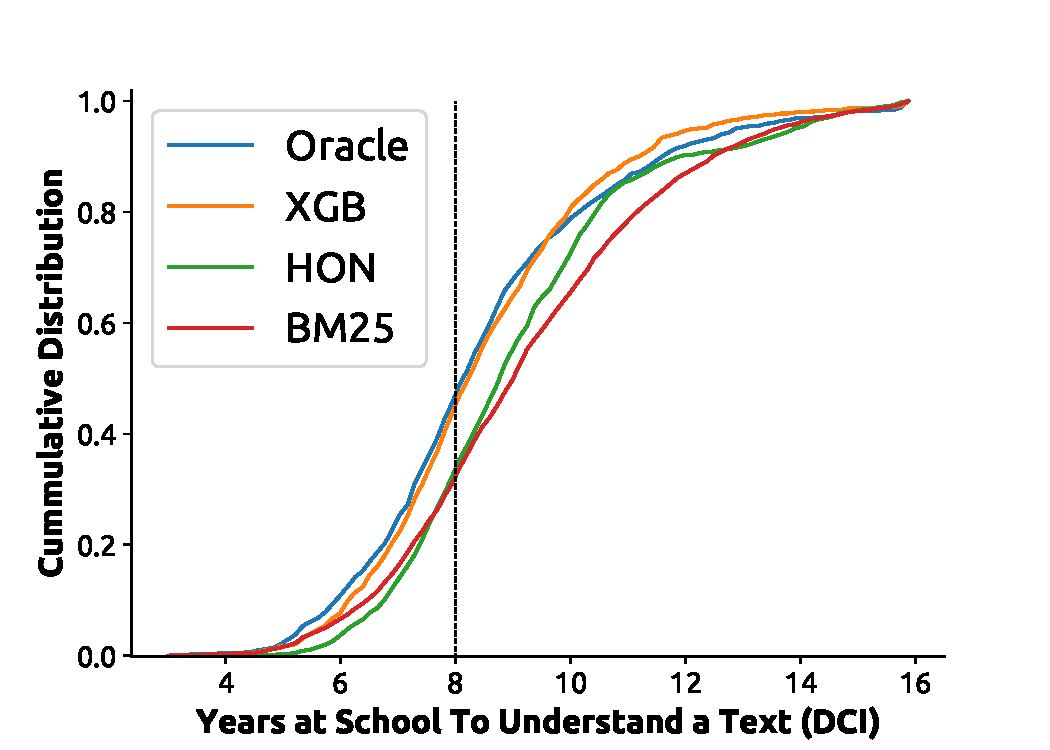
\includegraphics[width=.51\textwidth]{graphics/cumdist}
    %\vspace{-0.2cm}
    \caption{Distribution of Dale-Chall Index (DCI) of search results. DCI measures the years of schooling required to understand a document. The average US resident reads at or below an 8th grade level (dashed line)\cite{cowan04,wallace04,davis04,stossel12}, which is the level suggested by NIH for health information on the Web~\cite{clear94}. The distribution for HON is similar to that of the baseline used in this article (BM25). Our best method (XGB) re-ranks documents to provide more understandable results; its distribution is similar to that of an ``Oracle'' system.}
   \label{fig:dist}
\end{figure}




% =================================================================================================================================== %
% =================================================================================================================================== %
% =================================================================================================================================== %


\subsection{Related Work}

\label{sec:related}
Understandability refers to the ease of comprehension of the information presented to a user. Put in other words, health information is understandable ``when consumers of diverse backgrounds and varying levels of health literacy can process and explain key messages''~\cite{shoemaker2014development}. Often the terms understandability and readability are used interchangeably: we use readability to refer to formulas that estimate how easy is to understand a text, usually based on its words and sentences. We use understandability to refer to the broader concept of ease of understanding: this is affected by text readability (as increasing readability tends to improve understanding), but may also be influenced by how legible a text is and its layout, including e.g., the use of images to explain difficult concepts.

There is a large body of literature that has examined the understandability of Web health content when the information seeker is a member of the general public. For example, Becker reported that the majority of health Web sites are not well designed for the elderly~\cite{becker04}, while Stossel et al. found that  health education material on the Web is not written at an adequate reading level~\cite{stossel12}. Zheng and Yu have reported on the readability of electronic health records compared to Wikipedia pages related to diabetes and found that readability measures often do not align with user ratings of readability~\cite{zheng2017readability}. 
A common finding of these studies is that, in general, health content available on Web pages is often hard to understand by the general public; this includes content that is retrieved in top ranked positions by current commercial search engines~\cite{graber99,fitzsimmons10,wiener13,patel13,meillier17}.

Previous Linguistics and Information Retrieval (IR) research has attempted to devise computational methods for the automatic estimation of text readability and understandability, and for the inclusion of these within search methods or their evaluation. Computational approaches to understandability estimations include (1) \textit{readability formulas}, which generally exploit word surface characteristics of the text, (2) \textit{machine learning} approaches, (3) matching with specialised \textit{dictionaries or terminologies}, often compiled with information about understandability difficulty.

Measures such as Coleman-Liau Index (CLI)~\cite{cli75}, Dale-Chall Index (DCI)~\cite{dale48} and Flesch Reading Easy (FRE)~\cite{flesch75}
%, Simple Measure of Gobbledygook~\cite{smog69} 
belong to the first category. These measures generally rely on surface-level characteristics of text, such as characters, syllables and word counts~\cite{dubay04}. While these measures have been widely used in studies investigating the understandability of health content retrieved by search engines (e.g.,~\cite{becker04,graber99,fitzsimmons10,stossel12,wiener13,patel13,meillier17}), 
%Palotti et al. found that they are heavily affected by the methods used to extract text from the HTML source~\cite{palotti15}. They were able to identify specific settings of an HTML preprocessing pipeline that provided consistent estimates. We shall revisit this work in more details in the Methods section, as we further investigate this problem by comparing the effect of HTML preprocessing on text understandability estimations in light of explicit human assessments. 
our preliminary work found that these measures are heavily affected by the methods used to extract text from the HTML source~\cite{palotti15}. We were able to identify specific settings of an HTML preprocessing pipeline that provided consistent estimates, but due to the lack of human assessments, we were not able investigate how well each HTML preprocessing pipeline correlated with human assessments.
We shall revisit and extend this work in more details in this article, as we further investigate this problem by comparing the effect of HTML preprocessing on text understandability estimations in light of explicit human assessments. 

The use of machine learning to estimate understandability forms an alternative approach. Earlier research explored the use of statistical natural language processing and language modelling~\cite{liu04,collins05,heilman07} as well as linguistic factors, such as syntactic features or lexical cohesion~\cite{pitler08}. While we replicated here many of the features devised in these works, they focus on estimating readability of general English documents rather than medical ones. In the medical domain, Zeng et al. explored features such as word frequency in different medical corpora to estimate concept familiarity, which prompted the construction of the Consumer Health Vocabulary (CHV)~\cite{zeng05,zeng06,zeng08}.  

The actual use of CHV or other terminologies such as the Medical Subject Headings (MeSH) belongs to the third category of approaches. The CHV is a prominent medical vocabulary dedicated to mapping layperson vocabulary to technical terms~\cite{zeng06}. It attributes a score for each of its concepts with respect to their difficulty, with lower/higher scores for harder/easier concepts. Researchers have evaluated CHV in tasks such as document analysis~\cite{leroy08} and medical expertise prediction~\cite{palotti14}.
The hierarchy of MeSH was previously used in the literature to identify hard concepts, assuming that a concept deep in the hierarchy is harder than a shallow one~\cite{yan11}. Other approaches combined vocabularies with word surface characteristics and syntactic features, like part of speech, into a unique readability measure~\cite{kim2007beyond}.

In this work, we investigated approaches to estimate understandability from each of these categories. We further extended Palotti et al.'s work to understand the influence of HTML preprocessing on automatic understandability methods and establish best practices. 

Some prior work has attempted to use understandability estimations for improving search results in consumer health search; as well as methods to evaluate retrieval systems that do account for understandability along with topical relevance. Palotti et al.~\cite{palotti2016ranking} have used learning to rank with standard retrieval features along with features based on readability formulas and medical lexical aspects to determine understandability. Van Doorn et al.~\cite{van2016balancing} have shown that learning a set of rankers that provide trade-offs across a number of relevance criteria, including readability/understandability, increases overall system effectiveness.   
Zuccon and Koopman~\cite{zuccon14}, and later Zuccon~\cite{zuccon2016understandability}, have proposed and investigated a family of measures based on the gain-discount framework, where the gain of a document is influenced by both its topical relevance and its understandability. They showed that, although generally correlated, topical-relevance evaluation alone provides differing system rankings compared to understandability-biased evaluation measures. 
In this work we further explored the development of retrieval methods that combine signals about topical relevance and understandability. 


